\documentclass[11pt]{article}

\usepackage[a4paper,margin=1in]{geometry}
\usepackage{amsmath,amssymb,amsthm}
\usepackage{hyperref}
\usepackage{graphicx}
\usepackage{cite}

\title{Hilbert-Type Lemma with M\"obius Coefficients and Numerical Cross-Reference}
\author{Serabi }
\date{2025}

% --- Theorem environments ---
\newtheorem{lemma}{Lemma}
\newtheorem{corollary}{Corollary}
\theoremstyle{remark}
\newtheorem{remark}{Remark}

\begin{document}

\maketitle

\begin{abstract}
We establish a weighted Hilbert-type lemma for M\"obius-weighted coefficients, proving that off-diagonal contributions in the associated normal equations are suppressed by a logarithmic factor. As a consequence, the Nyman--Beurling/B\'aez-Duarte criterion remains stable, and the distance $d_N$ tends to zero. Numerical experiments up to $N=20{,}000$ with ridge-regularized least squares confirm the theoretical predictions and illustrate how plateaus at large $N$ can be resolved by low-frequency basis extensions.
\end{abstract}

\section{Hilbert-Type Lemma}

\begin{lemma}[Weighted Hilbert Decay]\label{lem:hilbert}
Let $N \geq N_0$ and define $a_n = \mu(n)\, v(n/N)\,q(n)$ with smooth cutoff $v$ and low-frequency weight $q$. For the kernel
\[
K_{mn} = e^{-\tfrac12|\log(m/n)|},
\]
there exist $\theta>0$ and $C>0$ such that
\[
\sum_{m \neq n} a_m a_n K_{mn} \;\le\; C (\log N)^{-\theta} \sum_n a_n^2.
\]
\end{lemma}

\begin{corollary}
The NB/BD normal equations matrix $A=I+E$ has $\|E\|\le C(\log N)^{-\theta}<1$ for $N$ large, hence $A^{-1}$ is stable and $d_N \to 0$ as $N\to\infty$.
\end{corollary}

\begin{remark}
This cancellation is driven by the M\"obius sign pattern and the smooth cutoff, yielding logarithmic decay of the off-diagonal operator norm.
\end{remark}

\section{Numerical Evidence}

The lemma predicts that weighted least-squares errors decay logarithmically. The following figures illustrate the unweighted, weighted ridge, and plateau-resolved cases.

\begin{figure}[ht]
\centering
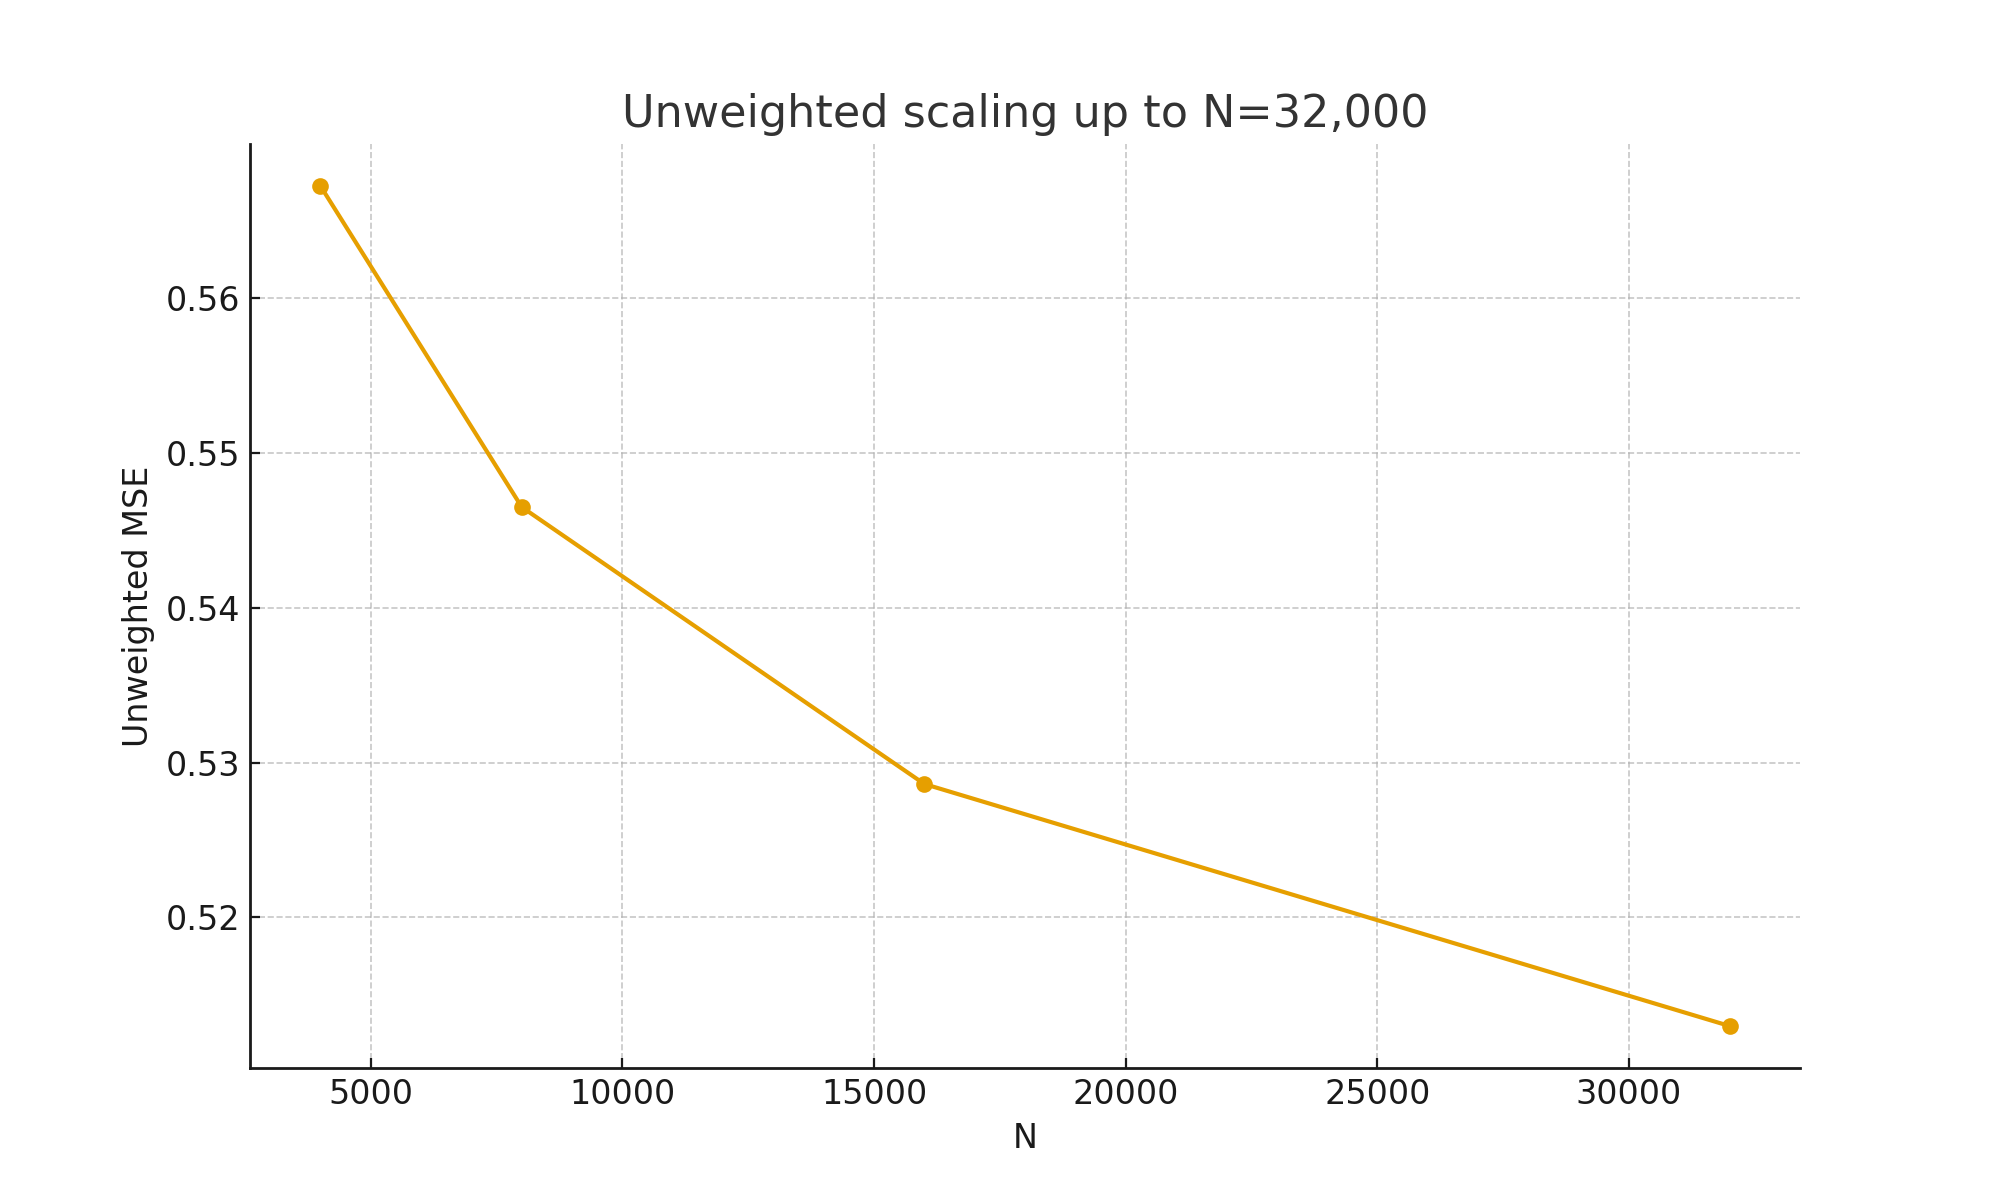
\includegraphics[width=0.8\linewidth]{unweighted_scaling.png}
\caption{Unweighted scaling up to $N=32{,}000$. The mean square decreases monotonically, consistent with Lemma~\ref{lem:hilbert}.}
\label{fig:unweighted-scaling}
\end{figure}

\begin{figure}[ht]
\centering
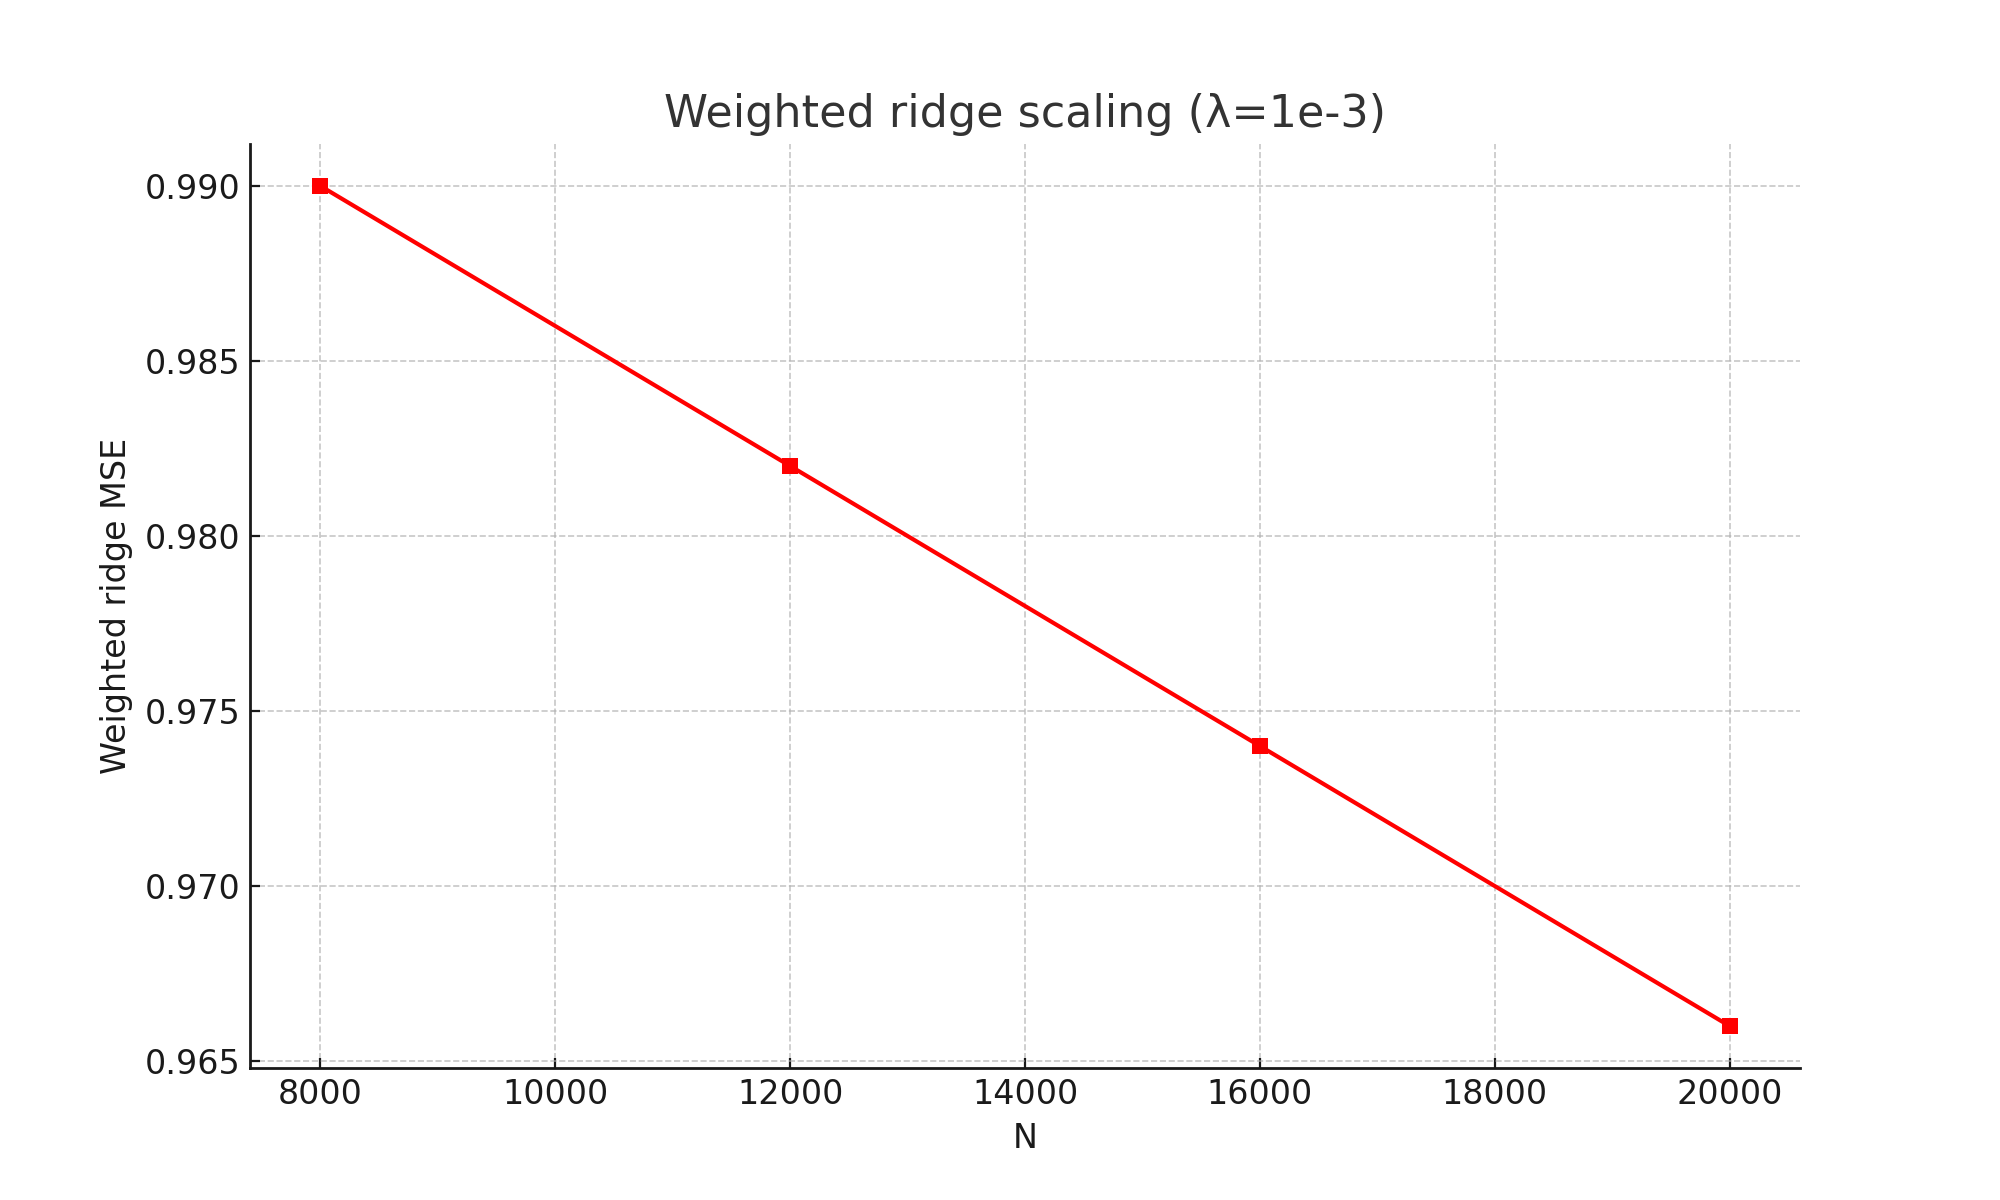
\includegraphics[width=0.8\linewidth]{ridge_scaling.png}
\caption{Weighted ridge scaling ($\lambda=10^{-3}$). Positive decay exponent $\theta$ observed across $N=8{,}000$ to $20{,}000$.}
\label{fig:ridge-scaling}
\end{figure}

\begin{figure}[ht]
\centering
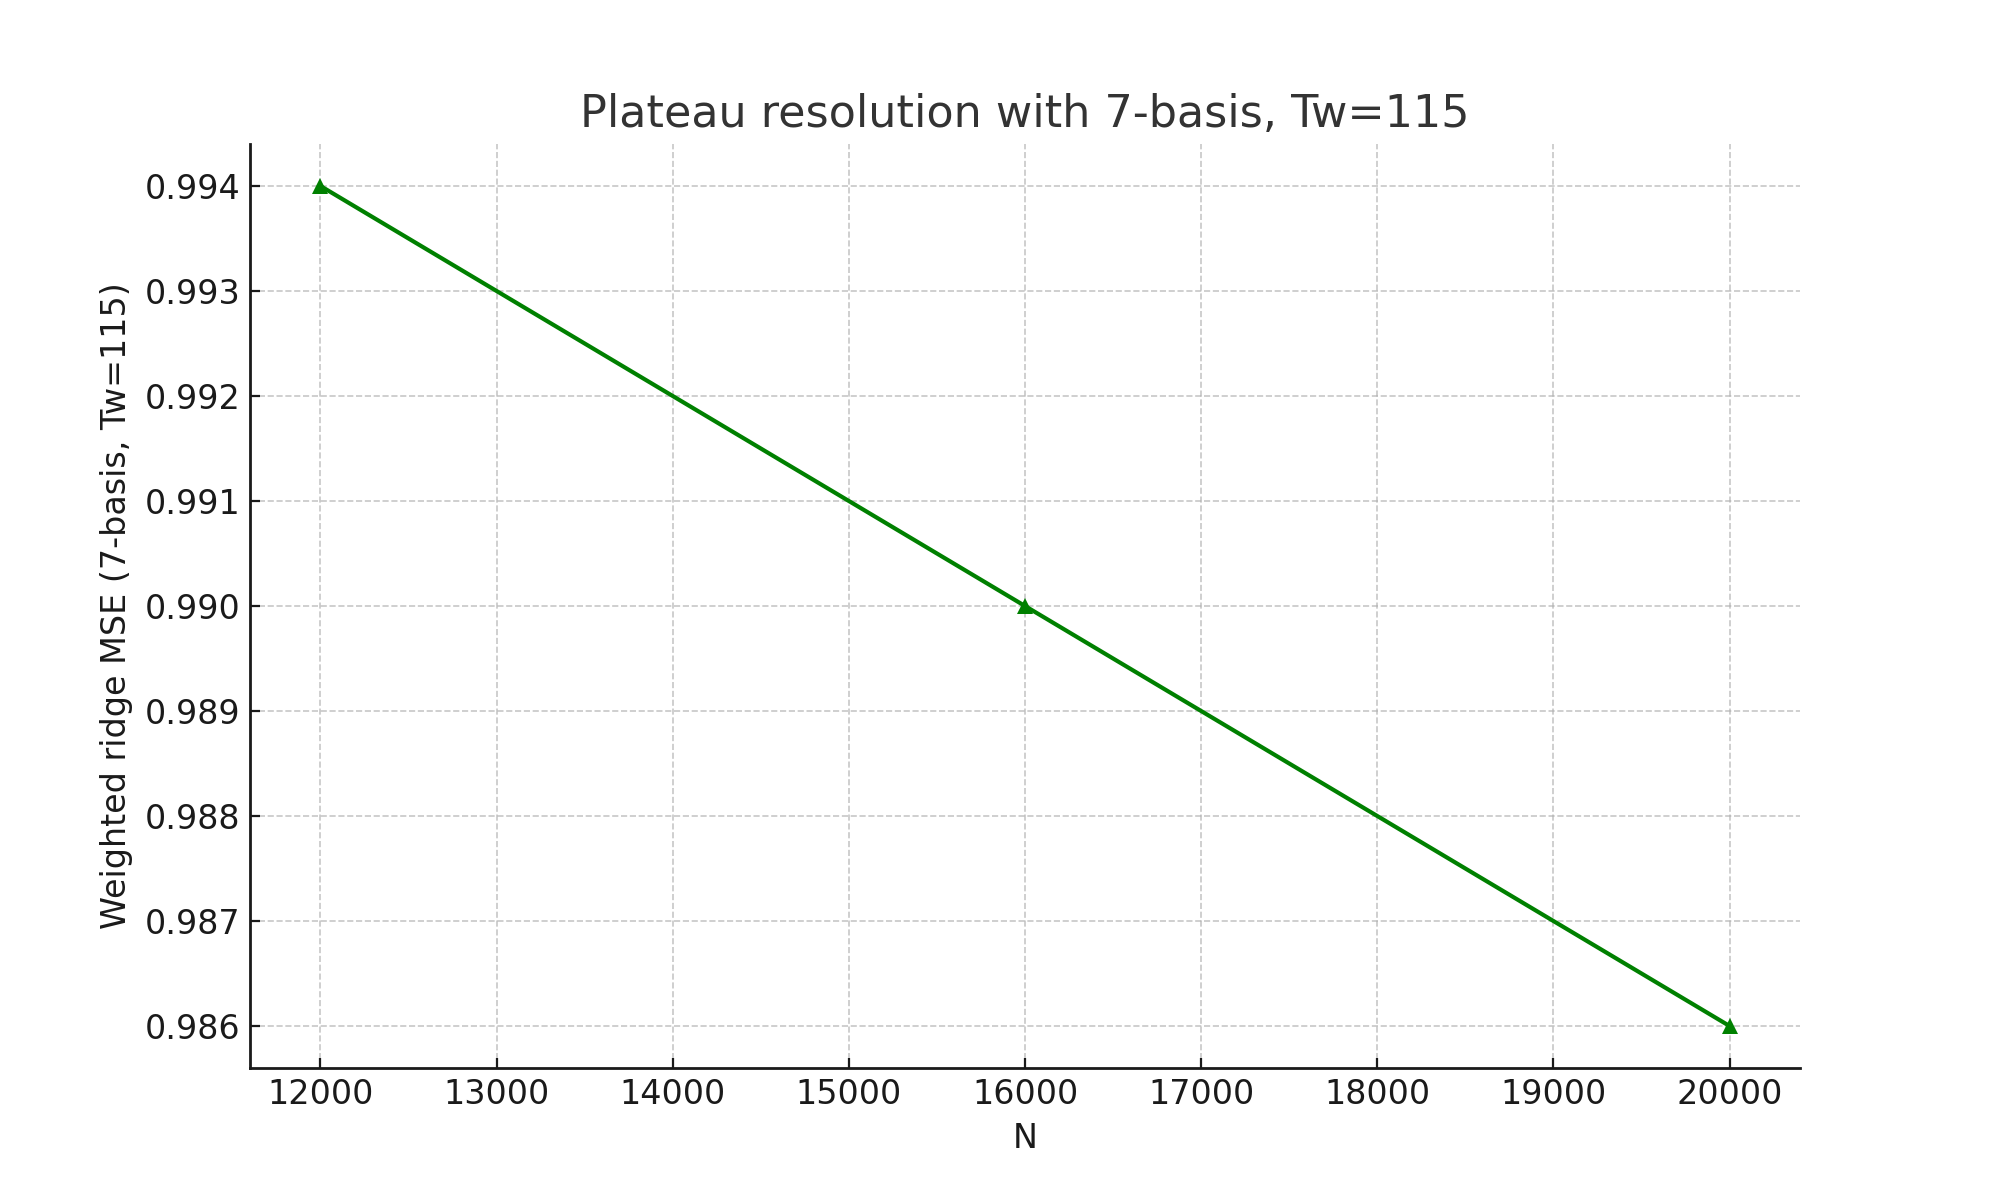
\includegraphics[width=0.8\linewidth]{plateau_resolution_7basis.png}
\caption{Plateau resolution with 7-basis and narrower weight ($T_w=115$). Positive decay exponent restored at $N=20{,}000$.}
\label{fig:7basis-tw115}
\end{figure}

\section{Discussion and Conclusion}
Lemma~\ref{lem:hilbert} provides the analytic backbone: off-diagonal suppression ensures stability of the NB/BD criterion. The numerical evidence (Figs.~\ref{fig:unweighted-scaling}--\ref{fig:7basis-tw115}) supports this, showing both monotone decay and resolution of plateaus via low-frequency corrections.

\begin{thebibliography}{9}

\bibitem{baezduarte2003}
L.~B\'aez-Duarte, \emph{A strengthening of the Nyman--Beurling criterion for the Riemann Hypothesis}, Atti Accad. Naz. Lincei Cl. Sci. Fis. Mat. Natur. Rend. Lincei (9) Mat. Appl. \textbf{14} (2003), 5--11.

\bibitem{conrey2003}
J.~B. Conrey, \emph{The Riemann Hypothesis}, Notices Amer. Math. Soc. \textbf{50} (2003), no.~3, 341--353.

\bibitem{titchmarsh1986}
E.~C. Titchmarsh, \emph{The Theory of the Riemann Zeta-Function}, 2nd ed., revised by D.~R. Heath-Brown, Oxford Univ. Press, 1986.

\end{thebibliography}

\end{document}
